\section{Implementation}\label{sec:impl}

The FFL runtime required an implementation that would translate specifications of augmentations to rendered HTML formulas. Figure~\ref{fig:dataflow} summarizes the translation process and the intermediate representations involved. Here, we briefly describe our implementation of augmentations in the FFL runtime in terms of each time the API is triggered.\footnote{\zed{Our implementation is hosted at \ifreview\textbf{[SEE CAMERA-READY VERSION]}\else\href{https://penn-hci.github.io/ffl}{\texttt{penn-hci.github.io/ffl}}\fi.}}

% \andrew{We should have 1--2 figures describing the parts of our implementation we think are most important for people to understand from our work. Here is my attempt at making a figure to try to describe the overall technical approach. I could also see having figures focusing specifically on aspects of the selector matching algorithm, or aspects related to how the HTML tree gets annotated.}

\begin{figure}
    \centering
    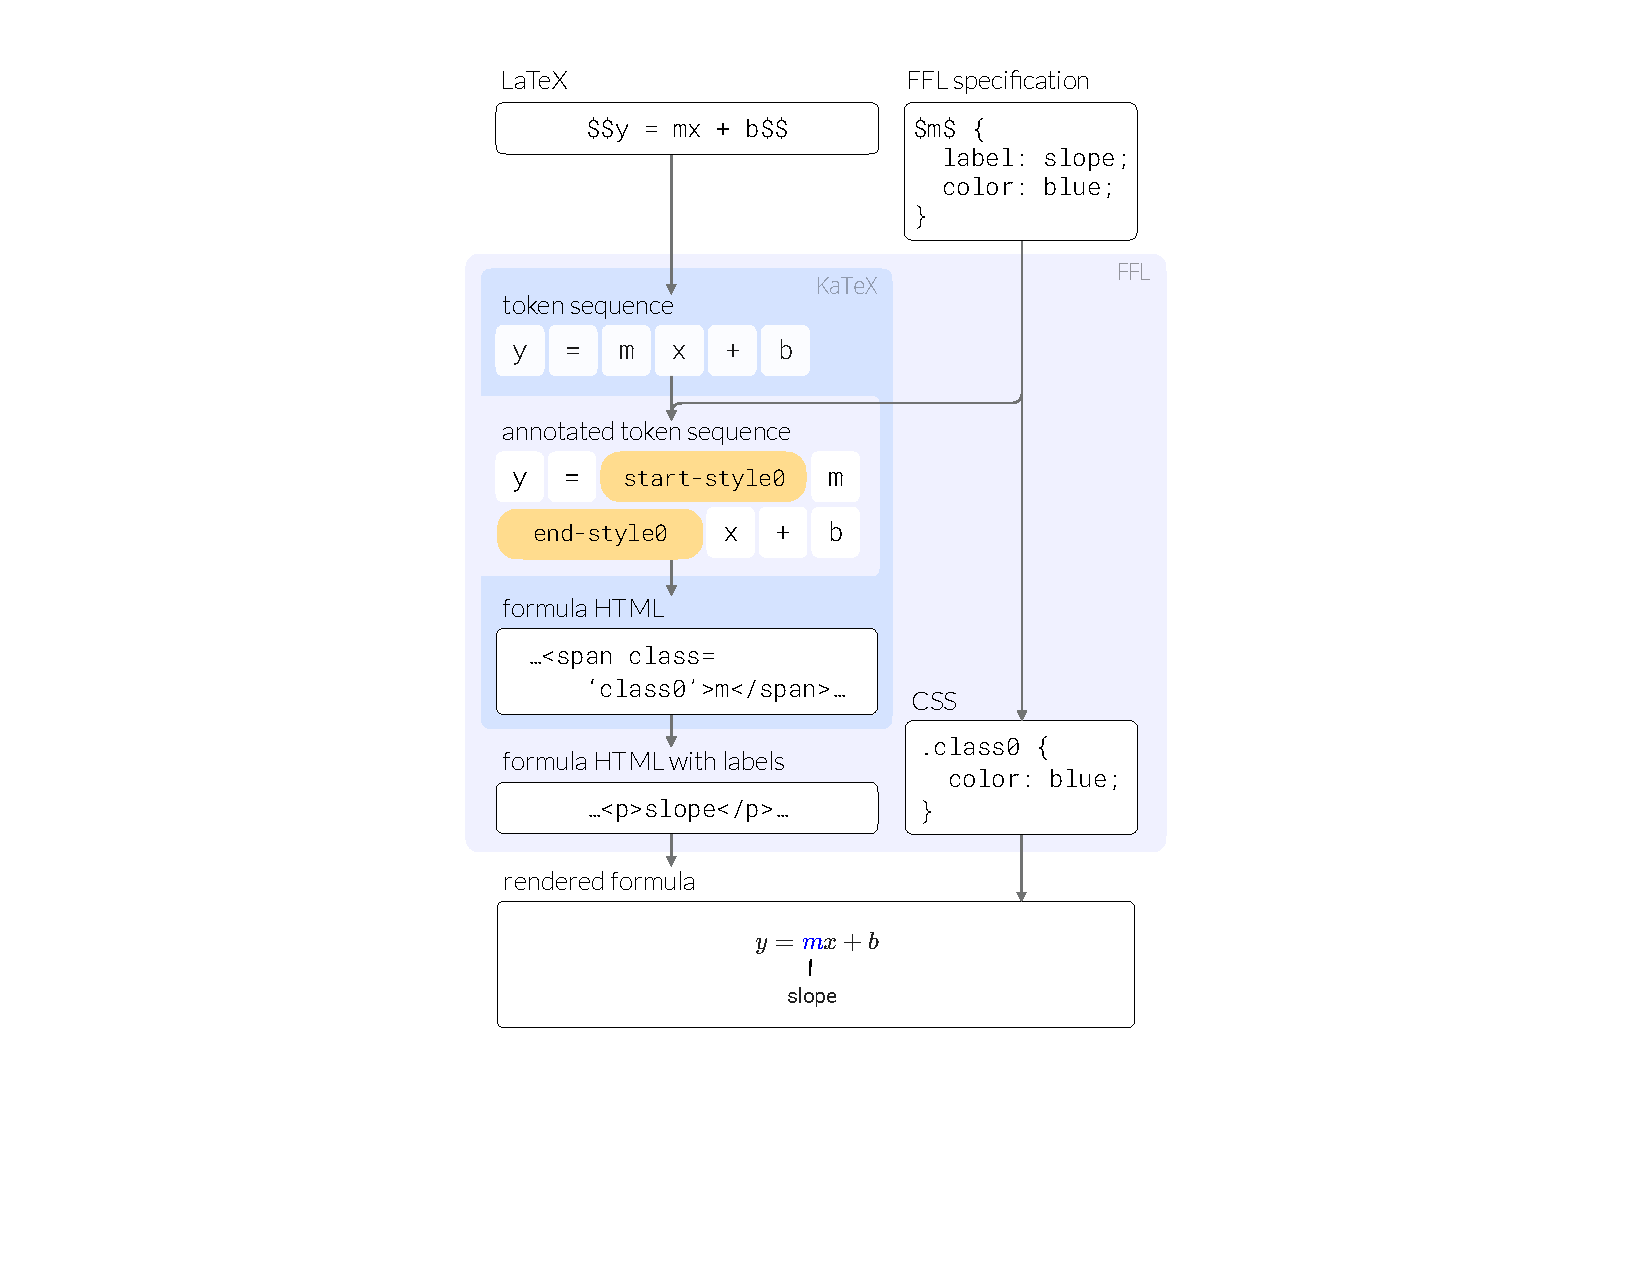
\includegraphics[width=.86\columnwidth]{figures/dataflow} 
    \caption{The generation of an augmented formula from LaTeX and an FFL style specification. \normalfont FFL wraps the  KaTeX library~\cite{tool:katex}, shimming itself into KaTeX's token parsing to detect and annotate expressions of interest. KaTeX generates an annotated HTML formula, which can be styled with CSS that FFL generates from its specification. FFL augments the generated HTML with labels by post-processing the generated HTML.}
    \Description{A decorative flowchart demonstrating how augmented formulas are generated from the LaTeX for a formula and an FFL style specification. The LaTeX math code and FFL style specification are passed into FFL, which then generates CSS from the FFL style specification and passes the LaTeX code to KaTeX, which FFL wraps. KaTeX tokenizes the LaTeX code and lets FFL insert marker tokens to indicate ranges where styles apply, linking the markers to generated CSS classes. KaTeX renders the token stream into HTML. FFL processes the HTML to add label elements. The HTML and CSS are rendered together as an augmented formula by the browser.}
    \label{fig:dataflow}
\end{figure}

% In general, we build on top of the \textit{KaTeX} renderer by both preprocessing
% the input \LaTeX\ and its options as well as postprocess its HTML output, while
% mostly relying on \textit{KaTeX}'s engine to process the \LaTeX\ itself. We choose
% to do this to depend on \textit{KaTeX}'s more robust support and maintenance.
% As seen in Figure \ref{fig:dataflow}, the pipeline is roughly as follows,

% The invocation is entirely handled by the editing environment.
% Here we use the sample editing environment we built where our \textit{markdown-it} integration
% calls the \textit{FFL} API on each formula and the global style specification. To achieve live preview, the below steps
% occurs each time it is called, although it is likely this could be optimized.

\subsection{Parsing the FFL specification}
FFL markup is parsed using a custom parser for the FFL grammar. The parser was generated by Peggy~\cite{Peggy}, a PEG parser generator, from an FFL grammar that resembles a subset of CSS grammar.

% First we parse FFL using \textit{Peggy}\cite{Peggy}, a PEG parser generator, where we define the grammar of our language.
% This allows us to make small modifications to our grammar on demand with minimal effort,
% as surface syntax change is often needed during our iterations. The rest of the process from this point on is syntax-agnostic.

\subsection{Matching LaTeX token sequences}
Next, the selectors are used to identify ranges of formula LaTeX that need to be augmented. To do this, we use KaTeX to lex both the selectors and the formula LaTeX into token sequences, with a small amount of parsing to normalize implicit groups. Then, we scan the LaTeX formula token stream for sub-sequences matching the selector, similarly tokenized by KaTeX. \zed{A segment and selector are considered matching if they contain a sequence of matching tokens. Literal tokens are considered matching if they are equal and wildcards \texttt{?} and \texttt{*} match either a single or a sequence of tokens respectively. 
% \andrew{I'm not sure I understand this second part, could it be clarified?}
} The current implementation of sub-sequence search permits matching overlapping sub-sequences, and wildcard matches for the character and sequence wildcards.

Once a matching sub-sequence is found, KaTeX must be told to augment the characters in that sub-sequence. To do this, we insert special tokens before and after the sub-sequence. These special tokens instruct KaTeX to insert temporary \texttt{span} tags with a generated class name around the expression in the rendered formula HTML. While it inserts these special tokens, FFL creates a map from FFL selectors to the selector-specific class names, from which it builds a CSS style sheet that applies FFL styles (e.g., color, font weight) to the expression in the rendered HTML formula.

% Selector matching is implemented to maximize the chance of forward compatibility.
\zed{We implement the search for matching sub-sequences of tokens in a way that does not require changing KaTeX's implementation. Our approach is to handle matching in a custom KaTeX macro that we wrap around each formula. With KaTeX, macros are defined as JavaScript functions. When KaTeX expands a macro, it does so by calling the corresponding JavaScript function, passing the function a sequence of tokens found in the macro's arguments. We wrote a custom macro that, when expanded by KaTeX, takes the tokens of the formula, searches for matching sub-sequences, modifies those sub-sequences as described in the paragraphs above, and returns the modified tokens to KaTeX for further processing.}

% More precisely, we 
% In particular, we implement sub-sequence search by wrapping the formula LaTeX in a macro \zed{which serves as the single entry point into KaTeX's pipeline for the FFL runtime to process and decorate the formula token stream. The invocation of this macro by KaTeX also accepts a modified token stream in return, which we utilize to denote styles applied to the formula. This also removes the need to fork or modify KaTeX's implementation in order to support FFL, maximizing the chance of forward compatibility.}
% \andrew{This is a good start, though some of the phrases that threw me off are: ``JavaScript-powered,'' ``normal command,'' ``compute its expansion,'' ``accepts and updated token sequence,'' ``programmatic macro.'' I think we need to find a way to de-jargon those phrases, because they will only have meaning to folks who are uncommonly familiar with LaTeX.}

% \subsection{Matching \& Inserting Marker Tokens}
% With our parsed abstract syntax as the primary data source, we then create a programmatic
% macro afforded by \textit{KaTeX} as part of our calling options, in which we wrap our \LaTeX\
% string during the invocation of its API. At this stage, \textit{KaTeX} will tokenize
% the \LaTeX\ and invoke our macro callback during its expansion, at which point we insert
% special tokens marking the start and end of selection ranges that require styling, which
% will then be passed on to \textit{KaTeX}'s internal HTML representation. This is chosen in lieu of using \textit{KaTeX}'s
% \texttt{\textbackslash htmlClass} or \texttt{\textbackslash htmlStyle} in order to enable
% overlapping selections, which would heavily restrict the power of \textit{FFL} selectors and increase the complexity for its validation.
% Currently, this is an na\"ive search through the entire token tree for all possible matches.
% This is also the point where we determine the escaped CSS class names for our selections
% and transpile all of our styles into a CSS style string.
% After this, we hand off back to \textit{KaTeX} again who will continue to render the
% expanded expression into HTML.

% \subsection{Processing Markers \& Applying Styles}
\subsection{Applying styles}
Once KaTeX produces the HTML for a rendered formula, FFL traverses the HTML to associate styles with matched expressions. FFL searches for the previously inserted \texttt{span}s, removing them and applying generated CSS class names to the HTML elements between them. Then, it appends the generated CSS (including color and font weight) to a ``\texttt{style}'' element in the DOM, which has the effect of styling the matched elements in the expression.

% . At the same time during the traversal,
% we apply the escaped CSS classes to the corresponding elements, which we then style
% by inserting previously obtained CSS string as a \texttt{style} element to the DOM
% representation, which could then be converted to an HTML string or the browser's
% representation depending on the API function invoked.

\subsection{Drawing overlays and underlays}\label{sec:overlays}
Finally, all remaining kinds of augmentations collected during the HTML tree traversal are applied, including labels and background colors. Labels are drawn as relatively positioned HTML elements on the margins of the formula inside an SVG~\cite{tool:svg} element. Label positions are determined by locating the position and outer bounding box of all tokens in its corresponding expression. Label positions are adjusted to reduce overlap by Labella~\cite{tool:labella}. The formula is padded with additional space so that labels do not occlude the surrounding text. Background colors are implemented as relatively positioned boxes placed behind the corresponding expression; this implementation is necessary to support background colors for selections whose constituent elements have a joined area that differs from the rectangular bounding box of the whole expression to ensure that there is only one background box, rather than multiple overlapping boxes for each character element in the expression.

% Finally, we draw labels and background colors as SVG overlays. Here we locate the to-be-styled elements with CSS selectors before finding their bounding box, with which we calculate the positions of the background color rectangles as well as the positions of their labels with \textit{Labella.js}\cite{Labella}. Additional margin is added around the orignal formula such that the overlays do not overlap with surrounding elements.

\subsection{Technical limitations}\label{tech-limitations}

Our current technical approach suffices for reifying the ideas behind FFL in a working tool. Here, we describe technical limitations that should be addressed to increase FFL's flexibility and robustness.

% \andrew{This is all great, though we should reduce it to half a column or less.}

% For parsing and rendering, we use existing versions of the {KaTeX} library to circumvent any duplicate, difficult, and likely error-bound venture in recreating a LaTeX parser. However, due to the lack of direct access to all phases of internal representations in KaTeX, the following functionalities are not trivial to implement following our current approach.

% \paragraph{Matching symbols that have both superscripts and subscripts} An author needs to know the order in which subscripts and superscripts were defined, even though this order could be changed while still achieving the same visual appearance of an expression.

\paragraph{Behavior of sequence wildcard} One revelation from our development was that the \texttt{glob}-style ``\texttt{*}'' wildcard is not well-defined for strings with the inherent hierarchy of LaTeX formulas. The current behavior of ``\texttt{*}'' is to match any terminal token or group at the same group level as the ``\texttt{*}'' in the selector. This decision remains to be more closely examined. % TODO: add back "violated expectations" if a good example is found

%% The current implementation of an unbounded wildcard also incurs a performance cost. \andrew{This is currently too hand-wavy---we need to make it more concrete (i.e., ``selector X on formula Y takes time T. This selector and formula is representative of the kinds of selectors people would commonly write with FFL. Parsing time increases to time T when selector X is used instead, showing that performance is influenced by\ldots{}'') I think we need to provide these details; they might get in the way here, so we could provide a very brief example and concrete time here, and then add additional details to the appendix.} \zed{Initial manual tests show that it can sometimes require around 40~\textit{ms} of matching and render time, up from the typical 15~\textit{ms} of a literal match. This could possibly add up and is undesirable in documents larger than those used in the lab study. We expect based on our current un-optimized implementation a few straightforward opportunities to speed up the render by some small constant factor, bringing it down within a more acceptable range, although the exact detail remains to be investigated.}

% \paragraph{Browser API dependency} Background colors and labels require programmatic access to bounding boxes of rendered elements. Such programmatic access is available in browser-based editing environment, but not in other Javascript-based editing environments that render markup in a server sandbox.

\paragraph{Block styles}
For some styles, FFL transpiles directly to CSS. For others like background color, border, and padding, FFL requires custom solutions. The default approach of FFL is to apply a style to all tokens separately in an expression. Rather, block styling augmentations---like padding---should apply to an expression in whole. To overcome this brittleness for block styling, we believe future versions of FFL should use KaTeX's render to MathML~\cite{tool:mathml} instead of HTML; MathML contains structures that can be more easily detected and augmented for these styles, and has become mainstream into most major browsers earlier this year.

\paragraph{Performance}
\zed{Preliminary tests on a commodity laptop show that rendering a formula with FFL takes tens of milliseconds (i.e., 35ms to augment ``$x$'' in the linear regression formula from the \hyperref[Demo]{demo section}). This runtime is imperceptible for single augmentations applied to single formulas. Our tests lead us to attribute latency to the time FFL takes to insert augmentation markers into KaTeX's token stream: latency increases as more matches are found in the formula (e.g., it takes 50ms to augment expressions matching ``\texttt{\$*\$}'' in the same demo formula). As the number of augmentations and formulas grow, adjustments will be required (e.g., optimizations, parallelization) for FFL to continue to deliver instant feedback.}

% \paragraph{Performance} \zed{The need for inserting markers between every element, needed to identify ``instances'' of matches to correctly implement ``selection-wise'' styles such as \texttt{background-color}, incurs a small amount of performance penalty. This is more pronounced in cases where there are a large number of matches, such as when a selector involves unbounded wildcards. Initial testing on a relatively performant personal machine showed that, including the \textasciitilde$30\,ms$ to render the document snippet from the 
% \hyperref[Demo]{demo section} takes without FFL, we found that coloring the selector \texttt{\$x\$} only takes around $35\,ms$ while \texttt{\$?\$} can take around $50\,ms$. While this has been sufficient for small documents and single formulas used in this study, especially given that wildcards are usually bounded by literal tokens, the effect of many selectors could still accumulate in large documents and is undesirable. We have identified several potential optimization opportunities which we suspect might speed up the rendering process by at least a small constant factor. We plan to investigate them and implement the change in the future.}

% It is possible that {MathML} could serve as that desired ``intermediate'' representation as well as the final output, which we decided against, as it was not widely supported at the time of implementation. Nonetheless, as of early 2023, this is rapidly changing and building on top of {MathML} might be an option worth exploring for re-implementation of {FFL}, which might make addressing some of the above issues less tedious.

% \paragraph{Off-browser rendering} For some annotations, we rely on browser API to determine the bounding boxes of rendered elements, which KaTeX does not usually require. This prevents us to integrate with both traditional LaTeX environments such as \texttt{pdflatex} as well as tools such as \textit{VS Code}~\cite{tool:vscode} which renders previews in a ``server'' sandbox.\\

% \label{mathml_integration}
% It is possible that {MathML} could serve as that desired ``intermediate'' representation as well as the final output, which we decided against, as it was not widely supported at the time of implementation. Nonetheless, as of early 2023, this is rapidly changing and building on top of {MathML} might be an option worth exploring for re-implementation of {FFL}, which might make addressing some of the above issues less tedious.